\hypertarget{node_8h}{
\section{src/node.h File Reference}
\label{node_8h}\index{src/node.h@{src/node.h}}
}
\hyperlink{classNode}{Node} class for graphical representation purposes. 



This graph shows which files directly or indirectly include this file:\nopagebreak
\begin{figure}[H]
\begin{center}
\leavevmode
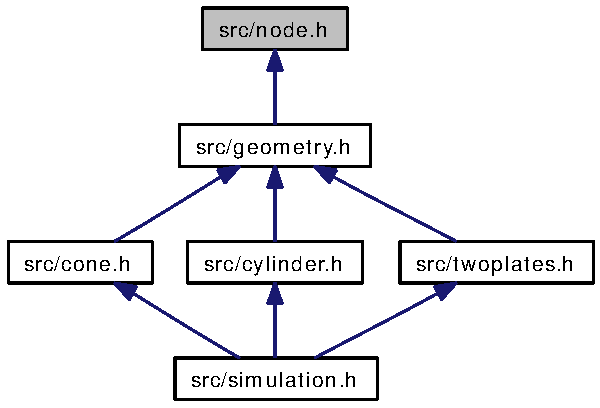
\includegraphics[width=162pt]{node_8h__dep__incl}
\end{center}
\end{figure}
\subsection*{Classes}
\begin{CompactItemize}
\item 
class \hyperlink{classNode}{Node}
\end{CompactItemize}


\subsection{Detailed Description}
\hyperlink{classNode}{Node} class for graphical representation purposes. 

Simple point definition and manipulation. It has a scalar property for storing the power density.

\begin{Desc}
\item[Author:]Daniel Iglesias $<$\href{mailto:daniel.iglesias@ciemat.es}{\tt daniel.iglesias@ciemat.es}$>$ \end{Desc}
